\documentclass{article}

\usepackage[english]{babel}
\usepackage[utf8]{inputenc}
\usepackage{amsmath,amssymb}
\usepackage{parskip}
\usepackage{graphicx}
\usepackage{listings}
\usepackage{float}

% Margins
\usepackage[top=2.5cm, left=3cm, right=3cm, bottom=4.0cm]{geometry}
% Colour table cells
\usepackage[table]{xcolor}

% Get larger line spacing in table
\newcommand{\tablespace}{\\[1.25mm]}
\newcommand\Tstrut{\rule{0pt}{2.6ex}}         % = `top' strut
\newcommand\tstrut{\rule{0pt}{2.0ex}}         % = `top' strut
\newcommand\Bstrut{\rule[-0.9ex]{0pt}{0pt}}   % = `bottom' strut

%%%%%%%%%%%%%%%%%
%     Title     %
%%%%%%%%%%%%%%%%%
\title{CSCI803 Assignment}
\author{Yao Xiao \\ SID 2019180015}
\date{\today}

\begin{document}
\maketitle

%%%%%%%%%%%%%%%%%
%   Problem 1   %
%%%%%%%%%%%%%%%%%
\section{Problem 1}
\subsection{Algorithm}
An algorithm is a finite set of instructions or logic, written in order, to accomplish a certain predefined task. Algorithm is not the complete code or program, it is just the core logic of a problem, which can be expressed either as an informal high level description as pseudocode or using a flowchart. 

In addition every algorithm satisfies the following properties: \textbf{Input, Output, Definiteness, Finiteness, Correctness}

\subsection{Data Structure}
In my view, a data structure is a specialized format for organizing, processing, retrieving and storing data. While there are several basic and advanced structure types, any data structure is designed to arrange data to suit a specific purpose so that it can be accessed and worked with in appropriate ways.

In computer programming, a data structure may be selected or designed to store data for the purpose of working on it with various algorithms. Each data structure contains information about the data values, relationships between the data and functions that can be applied to the data.



\section{Problem 2}
\begin{lstlisting}
import random

num_list = []

for i in range(0, 100):
    num = random.randint(0, 1000)
    num_list.append(num)

max_value = num_list[0]
for x in num_list:
    if x > max_value:
        max_value = x

min_value = num_list[0]
for i in num_list:
    if i < min_value:
        min_value = i

mean = sum(num_list) / len(num_list)

var = sum((x - mean)**2 for x in num_list) / len(num_list)

print("max value:", max(num_list))
print("min value:", min(num_list))
print("=========================")
print("max value:", max_value)
print("min value:", min_value)
print("mean value:", mean)
print("variance value:", var)
\end{lstlisting}


\begin{figure}[H]
    \centering
    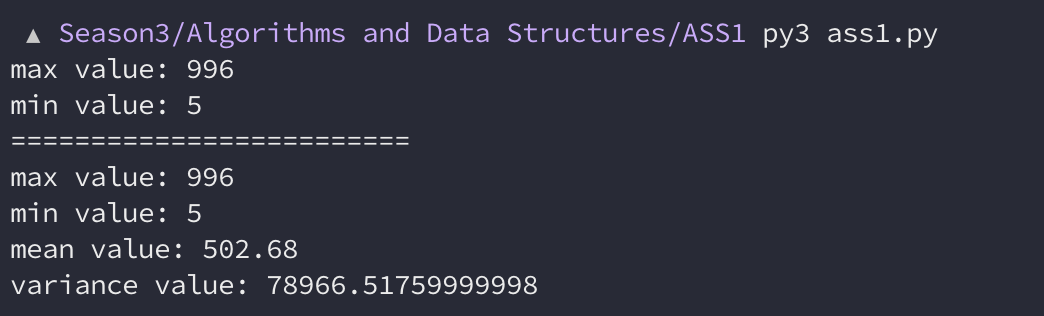
\includegraphics[width=1\textwidth]{Fig1.png}
\end{figure}

\end{document}
